% Options for packages loaded elsewhere
\PassOptionsToPackage{unicode}{hyperref}
\PassOptionsToPackage{hyphens}{url}
%
\documentclass[
]{article}
\usepackage{lmodern}
\usepackage{amssymb,amsmath}
\usepackage{ifxetex,ifluatex}
\ifnum 0\ifxetex 1\fi\ifluatex 1\fi=0 % if pdftex
  \usepackage[T1]{fontenc}
  \usepackage[utf8]{inputenc}
  \usepackage{textcomp} % provide euro and other symbols
\else % if luatex or xetex
  \usepackage{unicode-math}
  \defaultfontfeatures{Scale=MatchLowercase}
  \defaultfontfeatures[\rmfamily]{Ligatures=TeX,Scale=1}
\fi
% Use upquote if available, for straight quotes in verbatim environments
\IfFileExists{upquote.sty}{\usepackage{upquote}}{}
\IfFileExists{microtype.sty}{% use microtype if available
  \usepackage[]{microtype}
  \UseMicrotypeSet[protrusion]{basicmath} % disable protrusion for tt fonts
}{}
\makeatletter
\@ifundefined{KOMAClassName}{% if non-KOMA class
  \IfFileExists{parskip.sty}{%
    \usepackage{parskip}
  }{% else
    \setlength{\parindent}{0pt}
    \setlength{\parskip}{6pt plus 2pt minus 1pt}}
}{% if KOMA class
  \KOMAoptions{parskip=half}}
\makeatother
\usepackage{xcolor}
\IfFileExists{xurl.sty}{\usepackage{xurl}}{} % add URL line breaks if available
\IfFileExists{bookmark.sty}{\usepackage{bookmark}}{\usepackage{hyperref}}
\hypersetup{
  pdftitle={mia-rfid},
  hidelinks,
  pdfcreator={LaTeX via pandoc}}
\urlstyle{same} % disable monospaced font for URLs
\usepackage[margin=1in]{geometry}
\usepackage{color}
\usepackage{fancyvrb}
\newcommand{\VerbBar}{|}
\newcommand{\VERB}{\Verb[commandchars=\\\{\}]}
\DefineVerbatimEnvironment{Highlighting}{Verbatim}{commandchars=\\\{\}}
% Add ',fontsize=\small' for more characters per line
\usepackage{framed}
\definecolor{shadecolor}{RGB}{248,248,248}
\newenvironment{Shaded}{\begin{snugshade}}{\end{snugshade}}
\newcommand{\AlertTok}[1]{\textcolor[rgb]{0.94,0.16,0.16}{#1}}
\newcommand{\AnnotationTok}[1]{\textcolor[rgb]{0.56,0.35,0.01}{\textbf{\textit{#1}}}}
\newcommand{\AttributeTok}[1]{\textcolor[rgb]{0.77,0.63,0.00}{#1}}
\newcommand{\BaseNTok}[1]{\textcolor[rgb]{0.00,0.00,0.81}{#1}}
\newcommand{\BuiltInTok}[1]{#1}
\newcommand{\CharTok}[1]{\textcolor[rgb]{0.31,0.60,0.02}{#1}}
\newcommand{\CommentTok}[1]{\textcolor[rgb]{0.56,0.35,0.01}{\textit{#1}}}
\newcommand{\CommentVarTok}[1]{\textcolor[rgb]{0.56,0.35,0.01}{\textbf{\textit{#1}}}}
\newcommand{\ConstantTok}[1]{\textcolor[rgb]{0.00,0.00,0.00}{#1}}
\newcommand{\ControlFlowTok}[1]{\textcolor[rgb]{0.13,0.29,0.53}{\textbf{#1}}}
\newcommand{\DataTypeTok}[1]{\textcolor[rgb]{0.13,0.29,0.53}{#1}}
\newcommand{\DecValTok}[1]{\textcolor[rgb]{0.00,0.00,0.81}{#1}}
\newcommand{\DocumentationTok}[1]{\textcolor[rgb]{0.56,0.35,0.01}{\textbf{\textit{#1}}}}
\newcommand{\ErrorTok}[1]{\textcolor[rgb]{0.64,0.00,0.00}{\textbf{#1}}}
\newcommand{\ExtensionTok}[1]{#1}
\newcommand{\FloatTok}[1]{\textcolor[rgb]{0.00,0.00,0.81}{#1}}
\newcommand{\FunctionTok}[1]{\textcolor[rgb]{0.00,0.00,0.00}{#1}}
\newcommand{\ImportTok}[1]{#1}
\newcommand{\InformationTok}[1]{\textcolor[rgb]{0.56,0.35,0.01}{\textbf{\textit{#1}}}}
\newcommand{\KeywordTok}[1]{\textcolor[rgb]{0.13,0.29,0.53}{\textbf{#1}}}
\newcommand{\NormalTok}[1]{#1}
\newcommand{\OperatorTok}[1]{\textcolor[rgb]{0.81,0.36,0.00}{\textbf{#1}}}
\newcommand{\OtherTok}[1]{\textcolor[rgb]{0.56,0.35,0.01}{#1}}
\newcommand{\PreprocessorTok}[1]{\textcolor[rgb]{0.56,0.35,0.01}{\textit{#1}}}
\newcommand{\RegionMarkerTok}[1]{#1}
\newcommand{\SpecialCharTok}[1]{\textcolor[rgb]{0.00,0.00,0.00}{#1}}
\newcommand{\SpecialStringTok}[1]{\textcolor[rgb]{0.31,0.60,0.02}{#1}}
\newcommand{\StringTok}[1]{\textcolor[rgb]{0.31,0.60,0.02}{#1}}
\newcommand{\VariableTok}[1]{\textcolor[rgb]{0.00,0.00,0.00}{#1}}
\newcommand{\VerbatimStringTok}[1]{\textcolor[rgb]{0.31,0.60,0.02}{#1}}
\newcommand{\WarningTok}[1]{\textcolor[rgb]{0.56,0.35,0.01}{\textbf{\textit{#1}}}}
\usepackage{graphicx,grffile}
\makeatletter
\def\maxwidth{\ifdim\Gin@nat@width>\linewidth\linewidth\else\Gin@nat@width\fi}
\def\maxheight{\ifdim\Gin@nat@height>\textheight\textheight\else\Gin@nat@height\fi}
\makeatother
% Scale images if necessary, so that they will not overflow the page
% margins by default, and it is still possible to overwrite the defaults
% using explicit options in \includegraphics[width, height, ...]{}
\setkeys{Gin}{width=\maxwidth,height=\maxheight,keepaspectratio}
% Set default figure placement to htbp
\makeatletter
\def\fps@figure{htbp}
\makeatother
\setlength{\emergencystretch}{3em} % prevent overfull lines
\providecommand{\tightlist}{%
  \setlength{\itemsep}{0pt}\setlength{\parskip}{0pt}}
\setcounter{secnumdepth}{-\maxdimen} % remove section numbering

\title{mia-rfid}
\author{}
\date{\vspace{-2.5em}}

\begin{document}
\maketitle

loading in packages

\begin{Shaded}
\begin{Highlighting}[]
\KeywordTok{library}\NormalTok{(tidyverse)}
\end{Highlighting}
\end{Shaded}

loading in data

\begin{Shaded}
\begin{Highlighting}[]
\NormalTok{df1 <-}\StringTok{ }\KeywordTok{read_csv2}\NormalTok{(}\StringTok{"raw_data/Tracking/rawdata20210604.csv"}\NormalTok{)}
\NormalTok{df2 <-}\StringTok{ }\KeywordTok{read_csv2}\NormalTok{(}\StringTok{"raw_data/Tracking/rawdata20210605.csv"}\NormalTok{)}
\NormalTok{df3 <-}\StringTok{ }\KeywordTok{read_csv2}\NormalTok{(}\StringTok{"raw_data/Tracking/rawdata20210606.csv"}\NormalTok{)}
\NormalTok{df4 <-}\StringTok{ }\KeywordTok{read_csv2}\NormalTok{(}\StringTok{"raw_data/Tracking/rawdata20210607.csv"}\NormalTok{)}
\NormalTok{df5 <-}\StringTok{ }\KeywordTok{read_csv2}\NormalTok{(}\StringTok{"raw_data/Tracking/rawdata20210608.csv"}\NormalTok{)}
\NormalTok{df6 <-}\StringTok{ }\KeywordTok{read_csv2}\NormalTok{(}\StringTok{"raw_data/Tracking/rawdata20210609.csv"}\NormalTok{)}
\NormalTok{df7 <-}\StringTok{ }\KeywordTok{read_csv2}\NormalTok{(}\StringTok{"raw_data/Tracking/rawdata20210610.csv"}\NormalTok{)}
\end{Highlighting}
\end{Shaded}

stacking the data together

\begin{Shaded}
\begin{Highlighting}[]
\NormalTok{df <-}\StringTok{ }\KeywordTok{rbind}\NormalTok{(df1, df2, df3, df4, df5, df6, df7)}

\NormalTok{df}\OperatorTok{$}\NormalTok{data <-}\StringTok{ }\KeywordTok{as.character}\NormalTok{(df}\OperatorTok{$}\NormalTok{data)}

\NormalTok{df}
\end{Highlighting}
\end{Shaded}

creating milliseconds (ms) column

\begin{Shaded}
\begin{Highlighting}[]
\NormalTok{df}\OperatorTok{$}\NormalTok{date <-}\StringTok{ }\KeywordTok{format}\NormalTok{(}\KeywordTok{as.POSIXct}\NormalTok{(df}\OperatorTok{$}\NormalTok{datetimestamp,}\DataTypeTok{format=}\StringTok{"%d.%m.%Y %H:%M:%S:%OS"}\NormalTok{),}\StringTok{"%m.%d.%Y"}\NormalTok{)}
  
\NormalTok{df}\OperatorTok{$}\NormalTok{time <-}\StringTok{ }\KeywordTok{sub}\NormalTok{(}\StringTok{"^}\CharTok{\textbackslash{}\textbackslash{}}\StringTok{S+}\CharTok{\textbackslash{}\textbackslash{}}\StringTok{s+"}\NormalTok{, }\StringTok{''}\NormalTok{, df}\OperatorTok{$}\NormalTok{datetimestamp)}

\NormalTok{xx <-}\StringTok{ }\KeywordTok{strsplit}\NormalTok{(df}\OperatorTok{$}\NormalTok{time, }\DataTypeTok{split=}\StringTok{":"}\NormalTok{)}

\CommentTok{#xx}
\NormalTok{xxx <-}\StringTok{ }\KeywordTok{matrix}\NormalTok{(}\KeywordTok{unlist}\NormalTok{(xx), }\DataTypeTok{ncol =} \DecValTok{4}\NormalTok{, }\DataTypeTok{byrow =} \OtherTok{TRUE}\NormalTok{)}
\CommentTok{#xxx[,1]}
\CommentTok{#xxx[,2]}
\CommentTok{#xxx[,3]}
\CommentTok{#as.numeric(xxx[,4])}

\NormalTok{df}\OperatorTok{$}\NormalTok{ms<-}
\StringTok{  }\NormalTok{(}\DecValTok{3600000} \OperatorTok{*}\StringTok{ }\KeywordTok{as.numeric}\NormalTok{(xxx[,}\DecValTok{1}\NormalTok{])) }\OperatorTok{+}
\NormalTok{(}\DecValTok{60000} \OperatorTok{*}\StringTok{ }\KeywordTok{as.numeric}\NormalTok{(xxx[,}\DecValTok{2}\NormalTok{])) }\OperatorTok{+}
\NormalTok{(}\DecValTok{1000} \OperatorTok{*}\StringTok{ }\KeywordTok{as.numeric}\NormalTok{(xxx[,}\DecValTok{3}\NormalTok{])) }\OperatorTok{+}
\NormalTok{(}\DecValTok{1} \OperatorTok{*}\StringTok{ }\KeywordTok{as.numeric}\NormalTok{(xxx[,}\DecValTok{4}\NormalTok{]))}
\end{Highlighting}
\end{Shaded}

editing ms column to account for number days past

\begin{Shaded}
\begin{Highlighting}[]
\NormalTok{day_}\DecValTok{1}\NormalTok{ <-}\StringTok{ }\NormalTok{df }\OperatorTok\StringTok{ }\KeywordTok{filter}\NormalTok{(date }\OperatorTok{==}\StringTok{ "06.04.2021"}\NormalTok{)}

\NormalTok{  day_}\DecValTok{1}\OperatorTok{$}\NormalTok{ms <-}\StringTok{ }\KeywordTok{as.numeric}\NormalTok{(}\KeywordTok{unlist}\NormalTok{(day_}\DecValTok{1}\OperatorTok{$}\NormalTok{ms)) }\OperatorTok{-}\StringTok{ }\DecValTok{40089792}

\NormalTok{day_}\DecValTok{2}\NormalTok{ <-}\StringTok{ }\NormalTok{df }\OperatorTok\StringTok{ }\KeywordTok{filter}\NormalTok{(date }\OperatorTok{==}\StringTok{ "06.05.2021"}\NormalTok{)}

\NormalTok{  day_}\DecValTok{2}\OperatorTok{$}\NormalTok{ms <-}\StringTok{ }\NormalTok{(}\KeywordTok{as.numeric}\NormalTok{(}\KeywordTok{unlist}\NormalTok{(day_}\DecValTok{2}\OperatorTok{$}\NormalTok{ms)) }\OperatorTok{+}\StringTok{ }\NormalTok{(}\FloatTok{8.64e+7} \OperatorTok{*}\StringTok{ }\DecValTok{1}\NormalTok{)) }\OperatorTok{-}\StringTok{ }\DecValTok{40089792}

\NormalTok{day_}\DecValTok{3}\NormalTok{ <-}\StringTok{ }\NormalTok{df }\OperatorTok\StringTok{ }\KeywordTok{filter}\NormalTok{(date }\OperatorTok{==}\StringTok{ "06.06.2021"}\NormalTok{)}

\NormalTok{  day_}\DecValTok{3}\OperatorTok{$}\NormalTok{ms <-}\StringTok{ }\NormalTok{(}\KeywordTok{as.numeric}\NormalTok{(}\KeywordTok{unlist}\NormalTok{(day_}\DecValTok{3}\OperatorTok{$}\NormalTok{ms)) }\OperatorTok{+}\StringTok{ }\NormalTok{(}\FloatTok{8.64e+7} \OperatorTok{*}\StringTok{ }\DecValTok{2}\NormalTok{)) }\OperatorTok{-}\StringTok{ }\DecValTok{40089792}

\NormalTok{day_}\DecValTok{4}\NormalTok{ <-}\StringTok{ }\NormalTok{df }\OperatorTok\StringTok{ }\KeywordTok{filter}\NormalTok{(date }\OperatorTok{==}\StringTok{ "06.07.2021"}\NormalTok{)}

\NormalTok{  day_}\DecValTok{4}\OperatorTok{$}\NormalTok{ms <-}\StringTok{ }\NormalTok{(}\KeywordTok{as.numeric}\NormalTok{(}\KeywordTok{unlist}\NormalTok{(day_}\DecValTok{4}\OperatorTok{$}\NormalTok{ms)) }\OperatorTok{+}\StringTok{ }\NormalTok{(}\FloatTok{8.64e+7} \OperatorTok{*}\StringTok{ }\DecValTok{3}\NormalTok{)) }\OperatorTok{-}\StringTok{ }\DecValTok{40089792}

\NormalTok{day_}\DecValTok{5}\NormalTok{ <-}\StringTok{ }\NormalTok{df }\OperatorTok\StringTok{ }\KeywordTok{filter}\NormalTok{(date }\OperatorTok{==}\StringTok{ "06.08.2021"}\NormalTok{)}

\NormalTok{  day_}\DecValTok{5}\OperatorTok{$}\NormalTok{ms <-}\StringTok{ }\NormalTok{(}\KeywordTok{as.numeric}\NormalTok{(}\KeywordTok{unlist}\NormalTok{(day_}\DecValTok{5}\OperatorTok{$}\NormalTok{ms)) }\OperatorTok{+}\StringTok{ }\NormalTok{(}\FloatTok{8.64e+7} \OperatorTok{*}\StringTok{ }\DecValTok{4}\NormalTok{)) }\OperatorTok{-}\StringTok{ }\DecValTok{40089792}
  
\NormalTok{day_}\DecValTok{6}\NormalTok{ <-}\StringTok{ }\NormalTok{df }\OperatorTok\StringTok{ }\KeywordTok{filter}\NormalTok{(date }\OperatorTok{==}\StringTok{ "06.09.2021"}\NormalTok{)}

\NormalTok{  day_}\DecValTok{6}\OperatorTok{$}\NormalTok{ms <-}\StringTok{ }\NormalTok{(}\KeywordTok{as.numeric}\NormalTok{(}\KeywordTok{unlist}\NormalTok{(day_}\DecValTok{6}\OperatorTok{$}\NormalTok{ms)) }\OperatorTok{+}\StringTok{ }\NormalTok{(}\FloatTok{8.64e+7} \OperatorTok{*}\StringTok{ }\DecValTok{5}\NormalTok{)) }\OperatorTok{-}\StringTok{ }\DecValTok{40089792}

\NormalTok{day_}\DecValTok{7}\NormalTok{ <-}\StringTok{ }\NormalTok{df }\OperatorTok\StringTok{ }\KeywordTok{filter}\NormalTok{(date }\OperatorTok{==}\StringTok{ "06.10.2021"}\NormalTok{)}

\NormalTok{  day_}\DecValTok{7}\OperatorTok{$}\NormalTok{ms <-}\StringTok{ }\NormalTok{(}\KeywordTok{as.numeric}\NormalTok{(}\KeywordTok{unlist}\NormalTok{(day_}\DecValTok{7}\OperatorTok{$}\NormalTok{ms)) }\OperatorTok{+}\StringTok{ }\NormalTok{(}\FloatTok{8.64e+7} \OperatorTok{*}\StringTok{ }\DecValTok{6}\NormalTok{)) }\OperatorTok{-}\StringTok{ }\DecValTok{40089792}

\NormalTok{df <-}\StringTok{ }\KeywordTok{rbind}\NormalTok{(day_}\DecValTok{1}\NormalTok{, day_}\DecValTok{2}\NormalTok{, day_}\DecValTok{3}\NormalTok{, day_}\DecValTok{4}\NormalTok{, day_}\DecValTok{5}\NormalTok{, day_}\DecValTok{6}\NormalTok{, day_}\DecValTok{7}\NormalTok{)}

\NormalTok{df}\OperatorTok{$}\NormalTok{ms <-}\StringTok{ }\KeywordTok{as.character}\NormalTok{(df}\OperatorTok{$}\NormalTok{ms)}

\KeywordTok{as.data.frame}\NormalTok{(df[}\DecValTok{37200}\OperatorTok{:}\DecValTok{37300}\NormalTok{, ])}
\end{Highlighting}
\end{Shaded}

comparing \texttt{cantimestamp} with \texttt{milliseconds}

\begin{Shaded}
\begin{Highlighting}[]
\KeywordTok{plot}\NormalTok{(df}\OperatorTok{$}\NormalTok{cantimestamp, }\DataTypeTok{type =} \StringTok{"l"}\NormalTok{)}
\end{Highlighting}
\end{Shaded}

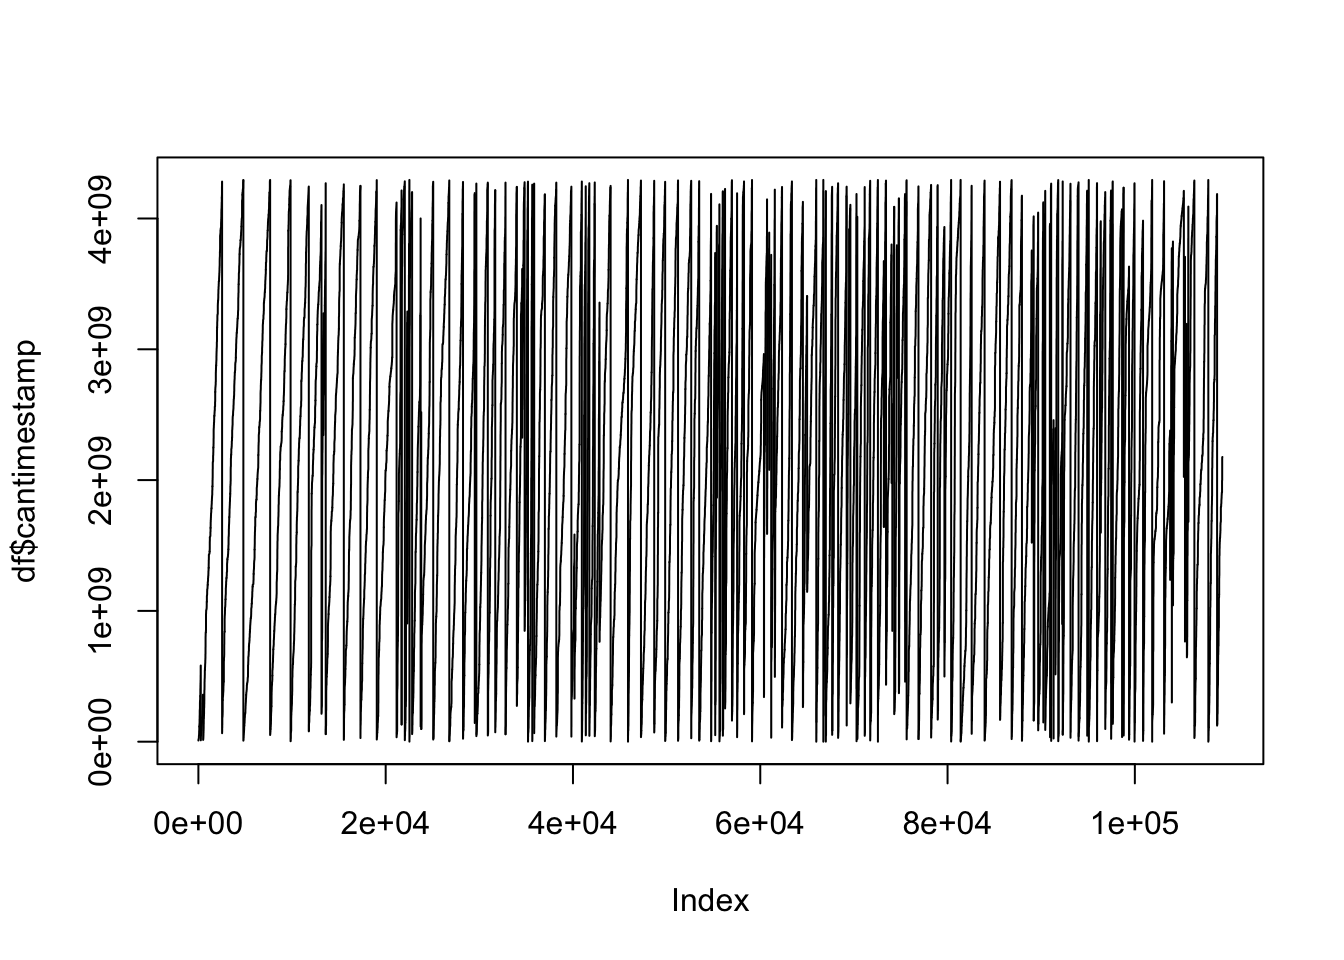
\includegraphics{mia-rfid_files/figure-latex/unnamed-chunk-6-1.pdf}

\begin{Shaded}
\begin{Highlighting}[]
\KeywordTok{plot}\NormalTok{(df}\OperatorTok{$}\NormalTok{ms, }\DataTypeTok{type =} \StringTok{"l"}\NormalTok{)}
\end{Highlighting}
\end{Shaded}

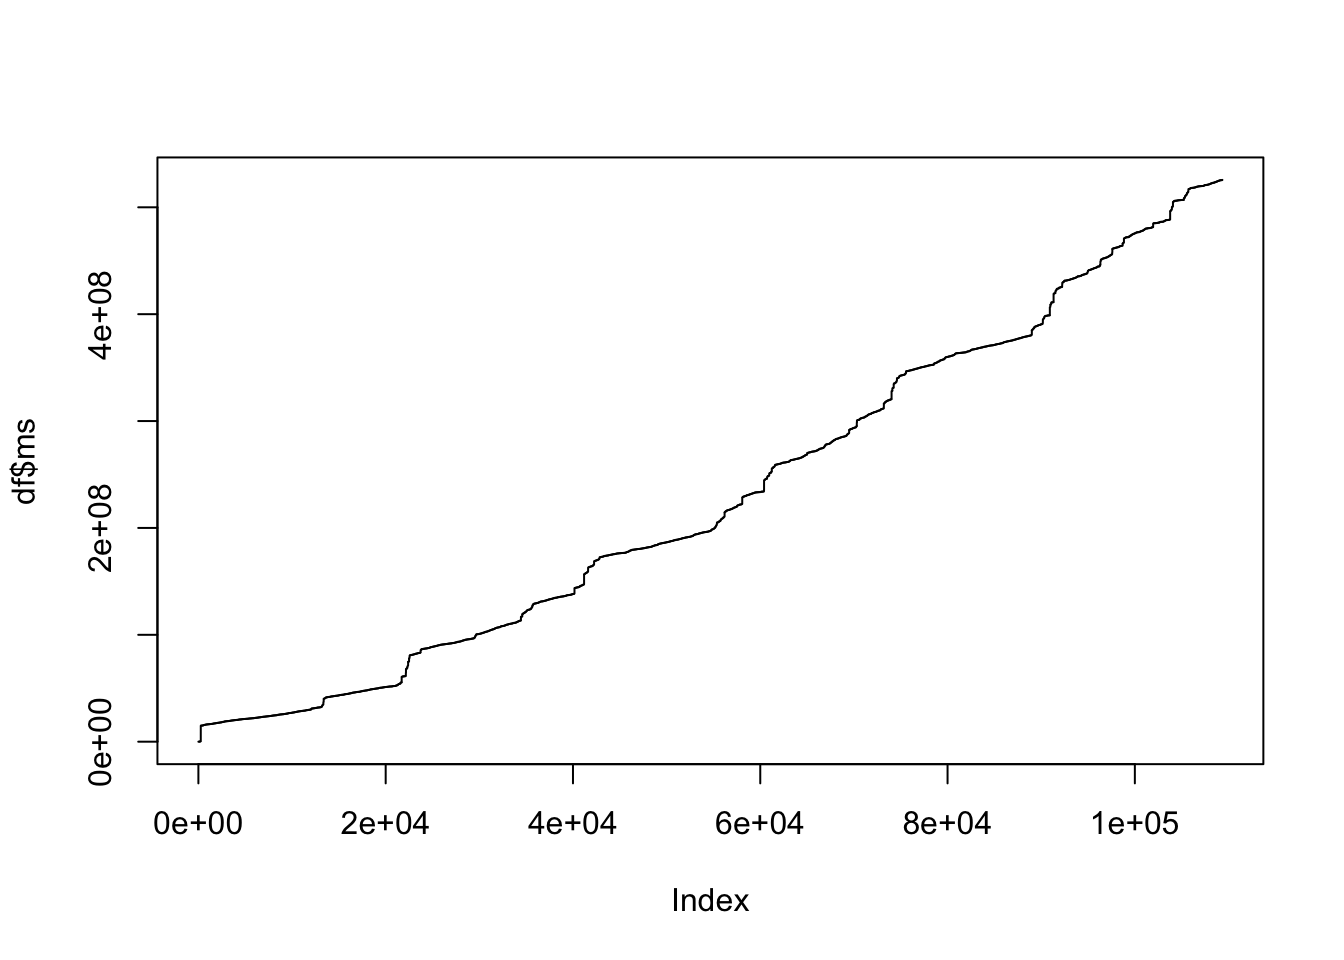
\includegraphics{mia-rfid_files/figure-latex/unnamed-chunk-6-2.pdf}

\begin{Shaded}
\begin{Highlighting}[]
\KeywordTok{head}\NormalTok{(df)}
\end{Highlighting}
\end{Shaded}

\begin{verbatim}
## # A tibble: 6 x 8
##   cantimestamp datetimestamp    deviceid antennaID data     date    time   ms   
##          <dbl> <chr>               <dbl>     <dbl> <chr>    <chr>   <chr>  <chr>
## 1      8969977 04.06.2021 11:0~       17         2 9001330~ 06.04.~ 11:08~ 0    
## 2      9763364 04.06.2021 11:0~       17         2 <NA>     06.04.~ 11:08~ 523  
## 3      9818886 04.06.2021 11:0~       17         2 9001330~ 06.04.~ 11:08~ 560  
## 4     10247875 04.06.2021 11:0~       17         1 9001330~ 06.04.~ 11:08~ 846  
## 5     10267878 04.06.2021 11:0~       17         2 <NA>     06.04.~ 11:08~ 859  
## 6     10893158 04.06.2021 11:0~       17         1 <NA>     06.04.~ 11:08~ 1276
\end{verbatim}

\begin{Shaded}
\begin{Highlighting}[]
\NormalTok{df }\OperatorTok\StringTok{ }
\StringTok{  }\KeywordTok{group_by}\NormalTok{(date) }\OperatorTok
\StringTok{  }\KeywordTok{arrange}\NormalTok{(ms) }\OperatorTok
\StringTok{  }\KeywordTok{mutate}\NormalTok{(}\DataTypeTok{rowid=}\KeywordTok{row_number}\NormalTok{()) }\OperatorTok
\StringTok{  }\KeywordTok{ggplot}\NormalTok{(., }\KeywordTok{aes}\NormalTok{(}\DataTypeTok{x=}\NormalTok{rowid, }\DataTypeTok{y=}\NormalTok{cantimestamp)) }\OperatorTok{+}
\StringTok{  }\KeywordTok{geom_line}\NormalTok{() }\OperatorTok{+}
\StringTok{  }\KeywordTok{facet_wrap}\NormalTok{(}\OperatorTok{~}\NormalTok{date)}
\end{Highlighting}
\end{Shaded}

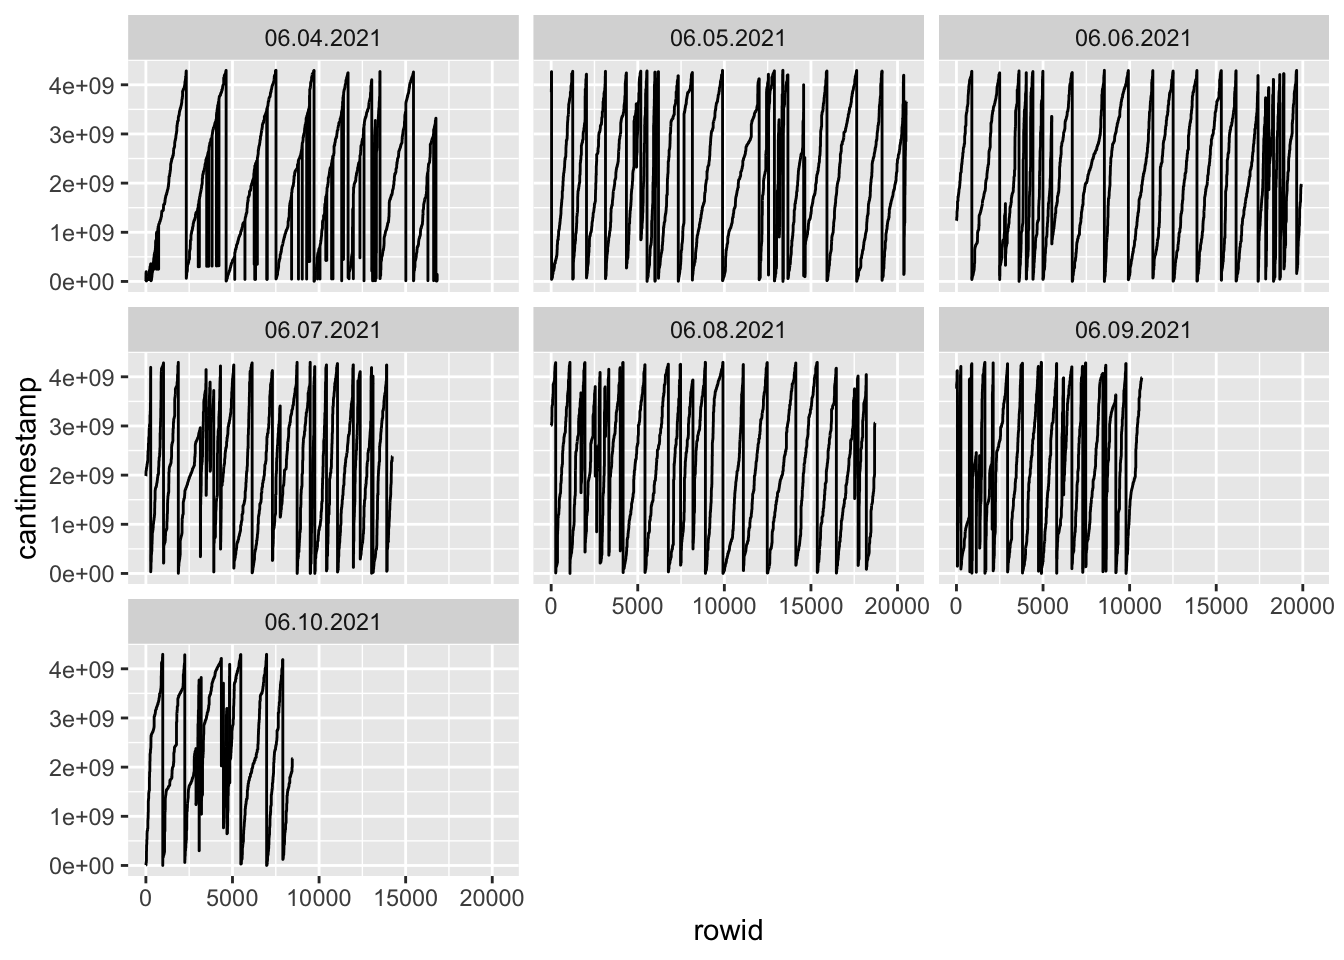
\includegraphics{mia-rfid_files/figure-latex/unnamed-chunk-7-1.pdf}

comparing cantimestamp restarting points to ms

\begin{Shaded}
\begin{Highlighting}[]
\KeywordTok{which}\NormalTok{(}\KeywordTok{lead}\NormalTok{(df}\OperatorTok{$}\NormalTok{cantimestamp)}\OperatorTok{<}\NormalTok{df}\OperatorTok{$}\NormalTok{cantimestamp) }\OperatorTok{+}\StringTok{ }\DecValTok{1} 
\end{Highlighting}
\end{Shaded}

\begin{verbatim}
##   [1]    255    509   2532   4803   7662   9845  11791  13147  13346  13380
##  [11]  13598  15530  17307  19049  21164  21699  22043  22153  22317  22499
##  [21]  22536  22823  23731  23799  25077  26794  28259  29513  29684  30906
##  [31]  31701  32798  34007  34587  34837  35197  35654  35859  37001  38222
##  [41]  39830  40162  40947  41367  41750  42256  42328  42838  44020  45875
##  [51]  47261  48675  49845  51221  52628  53481  54750  55190  55370  55642
##  [61]  56006  56242  56978  57526  58076  58266  59120  60394  60726  60957
##  [71]  61167  61233  61557  62326  63383  64554  65004  65981  66736  67001
##  [81]  67677  68313  69227  69491  69624  70280  70364  71154  71739  72564
##  [91]  73197  73429  74022  74102  74304  74596  74806  75467  75631  76895
## [101]  78245  78949  79665  80383  81399  82575  83956  85605  86844  87945
## [111]  89000  89200  89676  90227  90433  90948  91066  91322  91516  91821
## [121]  92237  92298  93129  93990  94913  95080  95963  96363  96843  97467
## [131]  97641  98635  98803  99379  99968 100876 101850 103122 103770 103950
## [141] 104070 105234 105354 105557 105717 106357 107847 108783
\end{verbatim}

\begin{Shaded}
\begin{Highlighting}[]
\NormalTok{drops <-}\StringTok{ }\NormalTok{df}\OperatorTok{$}\NormalTok{ms[}\KeywordTok{which}\NormalTok{(}\KeywordTok{lead}\NormalTok{(df}\OperatorTok{$}\NormalTok{cantimestamp)}\OperatorTok{<}\NormalTok{df}\OperatorTok{$}\NormalTok{cantimestamp) }\OperatorTok{+}\StringTok{ }\DecValTok{1}\NormalTok{ ]}

\NormalTok{drops <-}\StringTok{ }\KeywordTok{as.data.frame}\NormalTok{(}\KeywordTok{as.numeric}\NormalTok{(drops))}
\KeywordTok{colnames}\NormalTok{(drops) <-}\StringTok{ }\KeywordTok{c}\NormalTok{(}\StringTok{"delta_drops"}\NormalTok{)}

\NormalTok{drops <-}\StringTok{ }\KeywordTok{tail}\NormalTok{(drops, }\DecValTok{-1}\NormalTok{) }\OperatorTok{-}\StringTok{ }\KeywordTok{head}\NormalTok{(drops, }\DecValTok{-1}\NormalTok{)}

\KeywordTok{table}\NormalTok{(drops)}
\end{Highlighting}
\end{Shaded}

\begin{verbatim}
## drops
##   455631   523100   697443   882581  1162236  1186922  1256798  1498280 
##        1        1        1        1        1        1        1        1 
##  1621357  1761783  1862646  1878811  1920054  1956326  2024010  2058886 
##        1        1        1        1        1        1        1        1 
##  2099664  2109542  2238436  2299513  2299534  2355355  2522874  2532071 
##        1        1        1        1        1        1        1        1 
##  2569383  2605050  2644738  2670515  2712450  2724789  2765580  2778897 
##        1        1        1        1        1        1        1        1 
##  2782903  2796330  2796726  2799507  2801450  2809813  2812978  2813480 
##        1        1        1        1        1        1        1        1 
##  2820115  2822798  2825121  2825447  2828790  2831658  2833174  2834330 
##        1        1        1        1        1        1        1        1 
##  2839839  2844493  2844582  2847542  2847996  2848762  2851091  2853139 
##        1        1        1        1        1        1        1        1 
##  2853805  2854585  2854661  2855853  2856989  2859452  2860591  2862310 
##        1        1        1        1        1        1        1        1 
##  2862878  2863280  2863504  2863652  2864431  2864962  2865188  2865768 
##        1        1        1        1        1        1        1        1 
##  2866684  2867011  2871186  2871265  2872611  2875026  2876340  2876652 
##        1        1        1        1        1        1        1        1 
##  2879823  2879899  2886507  2886523  2887163  2888542  2892220  2892270 
##        1        1        1        1        1        1        1        1 
##  2894337  2897522  2898006  2901765  2901894  2903202  2904001  2913706 
##        1        1        1        1        1        1        1        1 
##  2921901  2926401  2928158  2943158  2945367  2953037  2954878  2969066 
##        1        1        1        1        1        1        1        1 
##  3008117  3031458  3034701  3040504  3083053  3089062  3189883  3190064 
##        1        1        1        1        1        1        1        1 
##  3324325  3344733  3450894  3460606  3518357  3553971  4073869  4283634 
##        1        1        1        1        1        1        1        1 
##  4576949  4957053  5201755  5302428  5647119  5705476  5724307  5737916 
##        1        1        1        1        1        1        1        1 
##  5767029  5767575  5802813  5865700  5920438  6150540  6221902  6737648 
##        1        1        1        1        1        1        1        1 
##  6789530  6821766  7094034  7290490  7520612  8553251  8602793  9374117 
##        1        1        1        1        1        1        1        1 
##  9618473 11485165 12285439 
##        1        1        1
\end{verbatim}

\begin{Shaded}
\begin{Highlighting}[]
\KeywordTok{hist}\NormalTok{(drops}\OperatorTok{$}\NormalTok{delta_drops)}
\end{Highlighting}
\end{Shaded}

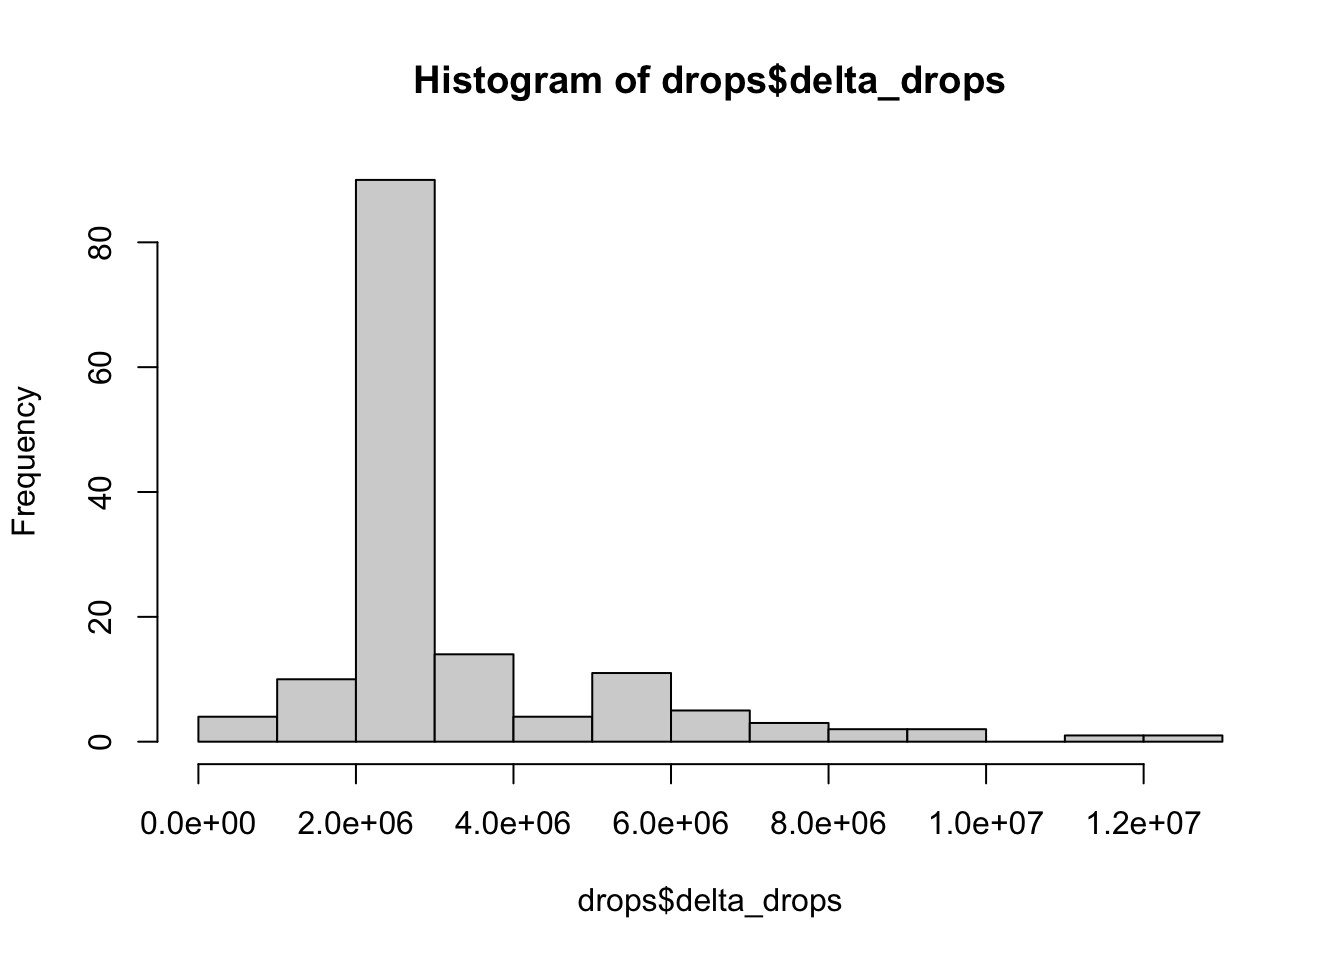
\includegraphics{mia-rfid_files/figure-latex/unnamed-chunk-8-1.pdf}

\begin{Shaded}
\begin{Highlighting}[]
\KeywordTok{hist}\NormalTok{(df}\OperatorTok{$}\NormalTok{cantimestamp)}
\end{Highlighting}
\end{Shaded}

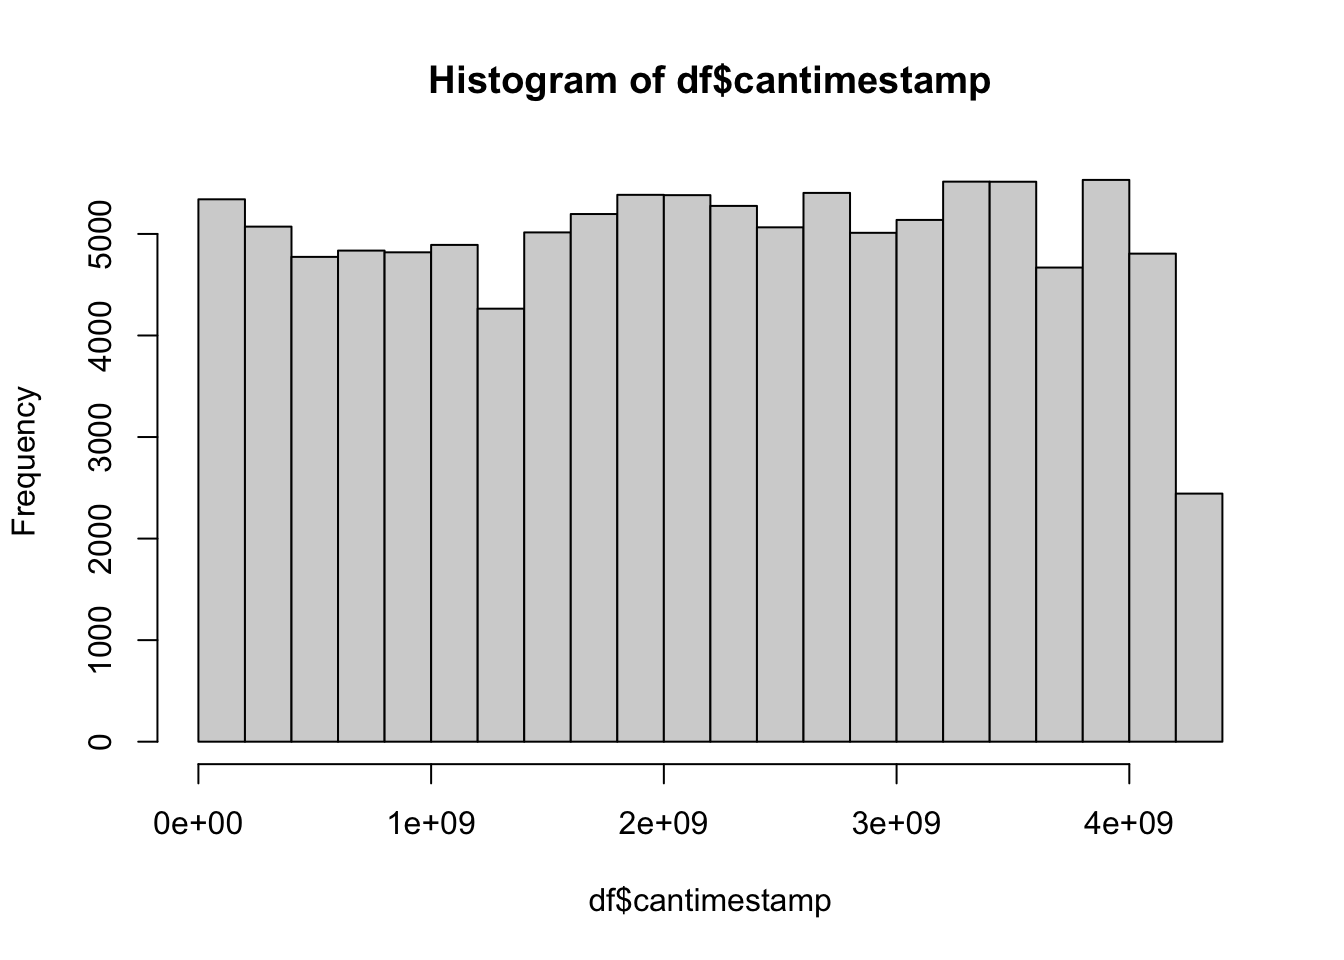
\includegraphics{mia-rfid_files/figure-latex/unnamed-chunk-8-2.pdf}

making a function to report impossible tube connections

\begin{Shaded}
\begin{Highlighting}[]
\NormalTok{tube_errors <-}\StringTok{ }\ControlFlowTok{function}\NormalTok{(df, }\DataTypeTok{pair1=}\KeywordTok{c}\NormalTok{(}\DecValTok{1}\NormalTok{,}\DecValTok{2}\NormalTok{), }\DataTypeTok{pair2=}\KeywordTok{c}\NormalTok{(}\DecValTok{3}\NormalTok{,}\DecValTok{4}\NormalTok{))\{}
  
\NormalTok{  ids <-}\StringTok{ }\KeywordTok{c}\NormalTok{(pair1,pair2)}
\NormalTok{  codes <-}\StringTok{ }\KeywordTok{c}\NormalTok{(}\StringTok{"3"}\NormalTok{,}\StringTok{"19"}\NormalTok{, }\StringTok{"17"}\NormalTok{, }\StringTok{"9"}\NormalTok{)}
  
\NormalTok{  x <-}\StringTok{ }\NormalTok{codes[}\KeywordTok{match}\NormalTok{(df}\OperatorTok{$}\NormalTok{deviceid, ids)]}
  
\NormalTok{  row.inds <-}
\StringTok{    }\KeywordTok{c}\NormalTok{(}\KeywordTok{intersect}\NormalTok{(}\KeywordTok{which}\NormalTok{(x }\OperatorTok{==}\StringTok{ "3"}\NormalTok{),}\KeywordTok{which}\NormalTok{(}\KeywordTok{lead}\NormalTok{(x) }\OperatorTok{==}\StringTok{ "19"} \OperatorTok{|}\StringTok{ }\KeywordTok{lag}\NormalTok{(x) }\OperatorTok{==}\StringTok{ "19"}\NormalTok{)),}
      \KeywordTok{intersect}\NormalTok{(}\KeywordTok{which}\NormalTok{(x }\OperatorTok{==}\StringTok{ "17"}\NormalTok{),}\KeywordTok{which}\NormalTok{(}\KeywordTok{lead}\NormalTok{(x) }\OperatorTok{==}\StringTok{ "9"} \OperatorTok{|}\StringTok{ }\KeywordTok{lag}\NormalTok{(x) }\OperatorTok{==}\StringTok{ "9"}\NormalTok{))}
\NormalTok{       )}
  
\NormalTok{  df}\OperatorTok{$}\NormalTok{error <-}\StringTok{ }\OtherTok{FALSE}
\NormalTok{  df[row.inds,}\StringTok{"error"}\NormalTok{]<-}\OtherTok{TRUE}
  
  \KeywordTok{return}\NormalTok{(df)}
\NormalTok{  \}}

\NormalTok{df <-}\StringTok{ }\KeywordTok{as.data.frame}\NormalTok{(}\KeywordTok{tube_errors}\NormalTok{(df, }\DataTypeTok{pair1 =} \KeywordTok{c}\NormalTok{(}\DecValTok{3}\NormalTok{,}\DecValTok{19}\NormalTok{), }\DataTypeTok{pair2 =} \KeywordTok{c}\NormalTok{(}\DecValTok{17}\NormalTok{,}\DecValTok{9}\NormalTok{)))}

\KeywordTok{filter}\NormalTok{(df, error}\OperatorTok{==}\OtherTok{TRUE}\NormalTok{)}
\end{Highlighting}
\end{Shaded}

dealing with NAs

\begin{Shaded}
\begin{Highlighting}[]
\NormalTok{df}\OperatorTok{$}\NormalTok{row <-}\StringTok{ }\DecValTok{1}\OperatorTok{:}\KeywordTok{nrow}\NormalTok{(df)}

\NormalTok{df}\OperatorTok{$}\NormalTok{ms <-}\StringTok{ }\KeywordTok{as.integer}\NormalTok{(df}\OperatorTok{$}\NormalTok{ms)}

\NormalTok{Match <-}\StringTok{ }\ControlFlowTok{function}\NormalTok{(row) \{}
  \KeywordTok{subset}\NormalTok{(df, deviceid }\OperatorTok{==}\StringTok{ }\NormalTok{df}\OperatorTok{$}\NormalTok{deviceid }\OperatorTok{&}\StringTok{ }
\StringTok{                }\NormalTok{antennaID }\OperatorTok{==}\StringTok{ }\NormalTok{df}\OperatorTok{$}\NormalTok{antennaID }\OperatorTok{&}
\StringTok{                }\NormalTok{row }\OperatorTok{>}\StringTok{ }\NormalTok{df}\OperatorTok{$}\NormalTok{row }\OperatorTok{&}
\StringTok{                }\KeywordTok{is.na}\NormalTok{(}\StringTok{"data"}\NormalTok{))[}\DecValTok{1}\NormalTok{, }\StringTok{"row"}\NormalTok{]}
\NormalTok{  \}}

\NormalTok{f <-}\StringTok{ }\ControlFlowTok{function}\NormalTok{(x) df[}\KeywordTok{c}\NormalTok{(}\KeywordTok{sapply}\NormalTok{(}\DecValTok{1}\OperatorTok{:}\KeywordTok{nrow}\NormalTok{(x), }\ControlFlowTok{function}\NormalTok{(i) }\KeywordTok{c}\NormalTok{(x}\OperatorTok{$}\NormalTok{row[i], }\KeywordTok{Match}\NormalTok{(x[i, ])))), ]}

\NormalTok{ddf <-}\StringTok{ }\KeywordTok{lapply}\NormalTok{(}\KeywordTok{split}\NormalTok{(df, df}\OperatorTok{$}\NormalTok{data), f)}
\end{Highlighting}
\end{Shaded}

\end{document}
